\documentclass{acmsiggraph}               % final

%% These two line bring in essential packages: ``mathptmx'' for Type 1
%% typefaces, and ``graphicx'' for inclusion of EPS figures.


\usepackage{graphicx}
\usepackage{url}
\usepackage{times}



%% Paper title.

\title{Simulate brushed metal surface in homegrown OpenGL render.}

%% Author / Affiliation (single author).

%%\author{Roy G. Biv}
%%\affiliation{Allied Widgets Research\thanks{email:roy.g.biv@aol.com}}

%% Author / Affiliation (multiple authors).

\author{Stefan Eng\thanks{e-mail: atn08sen@student.lth.se}
}
\affiliation{Lund University\\ Sweden}


%% Keywords that describe your work.
\keywords{OpenGL, from-scratch, brushed metal, C}

%%%%%% START OF THE PAPER %%%%%%

\begin{document}

\ifpdf
  \DeclareGraphicsExtensions{.jpg,.pdf,.mps,.png}
\else
  \DeclareGraphicsExtensions{.eps}
\fi


\maketitle

\begin{abstract}
The main motivation for the project is to get accustomed with the possibilities
and limitations of doing low level OpenGL programming from scratch in C. The projects
graphical focus is to simulate a brushed metal surface with semi-realistic light
reflections. \\

The final approach to the surface simulation includes a tangent-map texture to
simulate the topography texture of a brushed metal in combination with a
standard Phong shading model\cite{wiki_phong} to achieve the desired result.
Ideally this method would be compared to a more procedural approach in
combination with a slightly more advanced light model like the Blinn-Phong
model\cite{wiki_blinn}. This was never done due to the render backbone
implementation hitting a few problems and taking loger then anticipated.

\end{abstract}


\section{Introduction}

\begin{figure}[!ht]
    \centering
    
\includegraphics[width=0.7\columnwidth]{brushed.jpg}
    \caption{Photo of brushed metal.}
    \label{brushed_real}
\end{figure}

Brushed metal is a common type of metal texture on cookwares such as pots and
pans and can also be found on metallic counter tops. One of the more
recognizable properties of brushed metals is its ability to produce anisotropic
highlights due to the patterned surface area. \\

\begin{figure}[!ht]
    \centering
    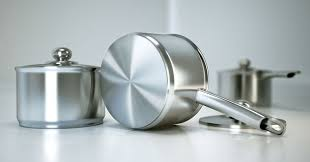
\includegraphics[width=0.7\columnwidth]{highlight.jpg}
    \caption{Example of anisotropic specular highlight.}
    \label{anisotropic_highlight}
\end{figure}

\section{Algorithms}
The main algorithm used for simulating bushed metal is \textit{Ward's model of
Anisotropic Reflection}\cite{GregWard}. \\

This model describes reflection in terms of a bidirectional reflectance
distribution function (BRDF), that describes how a light ray from any direction
is reflected into any other direction. Wards BRDF model incorporates to terms,
a diffuse reflectance term and a specular reflectance term.

\subsection{Diffuse term}

The diffuse term is a constant that equals $\frac{\rho_d}{\pi}$ where $\rho_d$
specifies the materials diffuse reflectance. Using the same BRDF
simplifications that are present in the Phong shading model, the specular terms
for the color wave lengths Red, Green and Blue can be reduced to pre-defined
material constants.

\subsection{Specular term}

\begin{figure}[!ht]
    \centering
    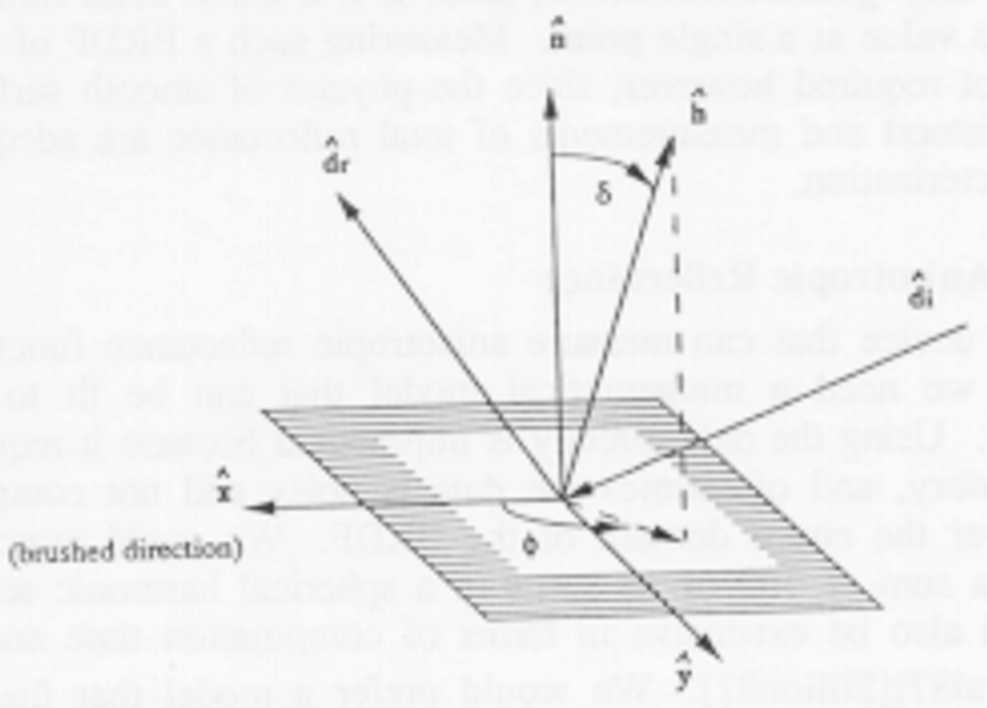
\includegraphics[width=0.7\columnwidth]{figure.png}
    \caption{Fig 5. from Greg Wards paper p. 268}
    \label{figure}
\end{figure}

By combining the vector setup with the following equation:

\begin{equation}
  \frac{\rho_d}{pi} + \rho_s \frac{1}{\sqrt{\cos{\theta_i},\cos{\theta_r}}}
  \frac{exp[-\tan^2\delta(\cos^2\phi/\alpha_x^2 +
  \sin^2\phi/\alpha_y^2)]}{4\pi\alpha_x\alpha_y}
\end {equation}

Where $\rho_d$ is the diffuse reflectance, $\rho_s$ is the specular
reflectance, $\alpha_x$ is the standard deviation of the surface slope in the
$\hat{x}$ direction. $\delta$ is the angle between the half vector $\hat{h}$
and the surface normal $\hat{n}$ and $\phi$ is the angle between the projection
of $\hat{h}$ projected into the plane and the $\hat{x}$ vector.
\\

By using normal the normalized vectors
\textbf{N},\textbf{V},\textbf{L},\textbf{T},\textbf{B},\textbf{H} for the
normal, view, light, binormal, tangent, and halfway vector, where the halfway vector
is defined as $\textbf{H} = (\textbf{V}+\textbf{L})/|\textbf{V}+\textbf{L}|$,
the earlier formula can then be restated as:
\begin{equation}
  \rho_s \frac{1}{\sqrt{(\textbf{L}\cdot\textbf{N})(\textbf{V}\cdot\textbf{N})}}
  \frac{1}{4\pi\alpha_x\alpha_y} exp (-2\frac{((\textbf{H}\cdot\textbf{T})/\alpha_x)^2)
((\textbf{H}\cdot\textbf{B})/\alpha_y)^2)} {1 + \textbf{H}\cdot\textbf{N}})
  %\sin^2\phi/\alpha_y^2)}{4\pi\alpha_x\alpha_y}
\end {equation}

and since $\rho_s$,$\alpha_x$ and $\alpha_y$ are all constants related to the
diffuse reflectance, they can be combined into the following equation:

\begin{equation}
  k_{specular} \frac{1}{\sqrt{(\textbf{L}\cdot\textbf{N})(\textbf{V}\cdot\textbf{N})}}
  exp (-2\frac{((\textbf{H}\cdot\textbf{T})/\alpha_x)^2)
((\textbf{H}\cdot\textbf{B})/\alpha_y)^2)} {1 + \textbf{H}\cdot\textbf{N}})
  %\sin^2\phi/\alpha_y^2)}{4\pi\alpha_x\alpha_y}
\end {equation}

\section{Written Report}

The report should be handed in an PDF format. You can use any word processing software you like, but you need to generate a PDF for the final submission.

The typesetting for this paper was done using pdf\LaTeX. It is recommended that you
use this as well, and therefore the ``source files'' for this very document are
available on the course website. If you are not familiar with pdf\LaTeX, then
you may use whatever other word processing program you like, as long as you mimic
the general style in this paper (i.e., you paper should look similar to
this paper).

The source files consists of two style files: \texttt{acmsiggraph.bst}
and \texttt{acmsiggraph.cls}, and these should be placed in the directory as the
files \texttt{project.tex} and \texttt{project.bib}. There is also a PNG image called
\texttt{lugg.png} that is shown later in this paper.
It is in \texttt{project.tex}, where you should delete this document's text,
and instead write your own text.

You should write your report as a scientific paper. It should have (at least)
the following sections:
\begin{itemize}
    \item Abstract [brief summary of key results]
    \item Introduction [why do what we did? motivation]
    \item Algorithms or Application [description of what you did, what algorithms you implemented]
    \item Results [e.g., performance, \textbf{screenshots}, usefulness etc]
    \item Discussion [what did not work, what worked well, what can be improved, optimizations you tried]
    \item Conclusion [any concluding remarks -- skip if you do not have anything to say in addition to what you've already said]
\end{itemize}
Some groups may not have enough important material to write a ``Discussion''-section,
and in such cases, that section can be omitted. Also, look at scientific papers,
%e.g.,~\cite{Hakura97,Igehy98,RaganKelley2011,Doggett2012,Ganestam2015}, and try to follow their general style.
When in doubt, come and ask us.
If you need references not found in the file \texttt{project.bib}, simply add your reference to
that file. The report should be 2--4 pages long.

You can include screenshots as PNGs or illustrations in the PDF format.
An example is shown in Figure~\ref{fig_lugg}. See the source file \texttt{project.tex}
for how this is done in \LaTeX.

\section{Conclusion}
Make a great project. You're clever. Surprise us (and the jury)!

\bibliographystyle{acmsiggraph}
\bibliography{project}
\end{document}
